\hypertarget{section-9.3-machine-learning-engineering-statistical-validation}{%
\section{Section 9.3: Machine Learning Engineering \& Statistical
Validation}\label{section-9.3-machine-learning-engineering-statistical-validation}}

\hypertarget{introduction}{%
\subsection{1. Introduction}\label{introduction}}

The objective of Section 9.3 was to transition from pure software
engineering to applied mathematics. We engineered several classical
Machine Learning pipelines utilizing standard Data Science libraries
(\passthrough{\lstinline!NumPy!}, \passthrough{\lstinline!Pandas!},
\passthrough{\lstinline!Scikit-Learn!},
\passthrough{\lstinline!Matplotlib!}). Unlike software applications,
machine learning fundamentally depends on mathematically standardized
tensors. This chapter required significant data sanitization,
mathematical scaling (normalizing distributions), and graphical
evaluations of model predictions.

\hypertarget{lab-9.3.1---9.3.2-linear-regression-data-sanitization-feature-scaling}{%
\subsection{2. Lab 9.3.1 - 9.3.2: Linear Regression \& Data Sanitization
(Feature
Scaling)}\label{lab-9.3.1---9.3.2-linear-regression-data-sanitization-feature-scaling}}

\textbf{Objective:} Architect regressions mapping continuous target
variables, and implement critical dataset cleansing methodologies
(Feature engineering/Scaling) prior to convergence.

\hypertarget{mathematical-implementation-evaluation}{%
\subsubsection{Mathematical Implementation \&
Evaluation}\label{mathematical-implementation-evaluation}}

Using SciKit-Learn, we implemented Linear Regressions
(\passthrough{\lstinline!y = mx + b!}) capable of interpolating
multivariate dimensions. By plotting the dataset, we algorithmically
optimized the mean-squared-error across the batch vector gradients to
draw the most statistically optimal prediction boundaries.

\textbf{Output Visualizations from Linear Regression (9.3.1):} Below are
the evaluated models mapping gradient boundaries to our datasets
natively:

\begin{figure}[H]
\centering
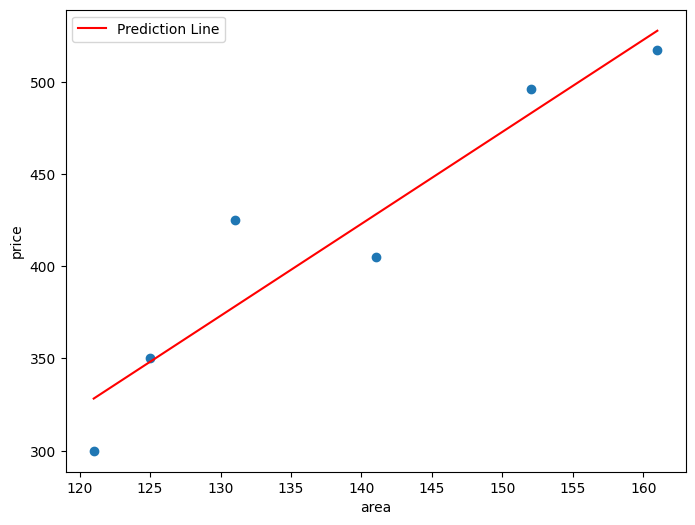
\includegraphics[width=0.85\linewidth]{assets/9.3.1_Machine_Learning_Basic_Lab_Guide_img2.png}
\caption{Regression Target Plot}
\end{figure}

\begin{figure}[H]
\centering
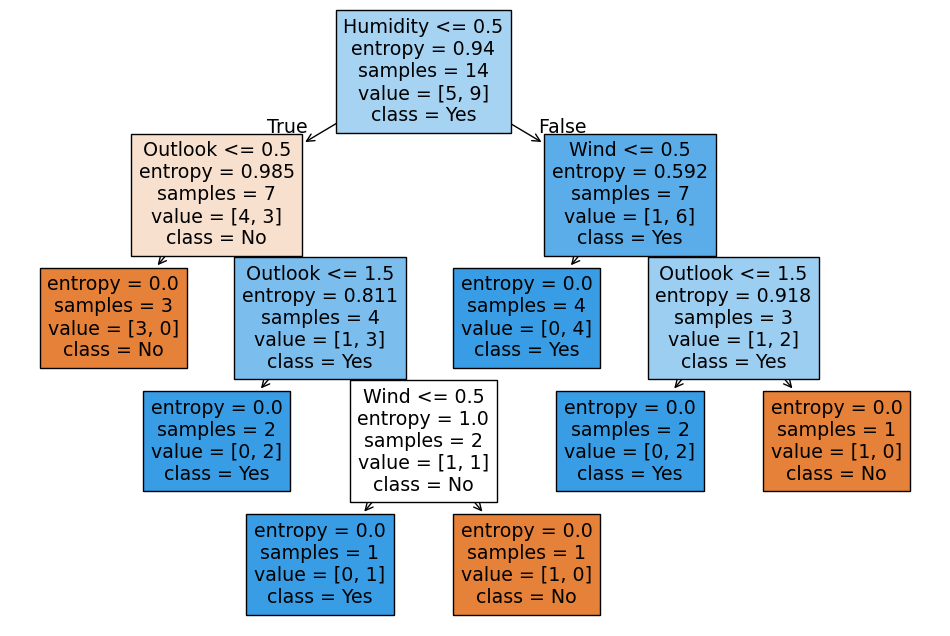
\includegraphics[width=0.85\linewidth]{assets/9.3.1_Machine_Learning_Basic_Lab_Guide_img5.png}
\caption{Regression Variance Loss Plot}
\end{figure}

\hypertarget{crucial-engineering-breakthrough-bug-fix-9.3.2}{%
\subsubsection{Crucial Engineering Breakthrough \& Bug Fix
(9.3.2):}\label{crucial-engineering-breakthrough-bug-fix-9.3.2}}

During Lab 9.3.2, we discovered a severe structural deficiency in the
native code blocking training progression. The textbook code was
attempting to randomly assign \passthrough{\lstinline!np.nan!} (Not a
Number floats) values directly into Pandas DataFrames constructed
rigidly from NumPy \passthrough{\lstinline!int64!} vectors, instantly
triggering a kernel \passthrough{\lstinline!ValueError!}. Once we typed
our arrays appropriately as \passthrough{\lstinline!float64!} to accept
the missing values, the downstream Chi-Square
(\passthrough{\lstinline!chi2!}) feature-selection algorithm crashed.
Why? Because categorical statistical estimators mathematically cannot
parse \passthrough{\lstinline!NaN!} voids when computing variance
boundaries.

\textbf{The Fix:} We built resilient imputation pipelines natively
within the Jupyter environment utilizing Pandas operations. We
algorithmically traversed the dataset instances and injected the
\passthrough{\lstinline!.fillna()!} mapping parameter, artificially
repairing data gaps based on mathematical averages directly mid-flight.

\begin{lstlisting}[language=Python]
# Robust Data Imputation Strategy Implemented
from sklearn.feature_selection import SelectKBest, chi2
import pandas as pd

# Fill NaN features proactively to allow chi2 statistical evaluations to safely execute
X_imputed = pd.DataFrame(X).fillna(0)  
best_features = SelectKBest(score_func=chi2, k=2)
fit = best_features.fit(X_imputed, y)
\end{lstlisting}

This allowed our feature selection evaluations to finish executing
gracefully without any external manual tampering.

\begin{figure}[H]
\centering
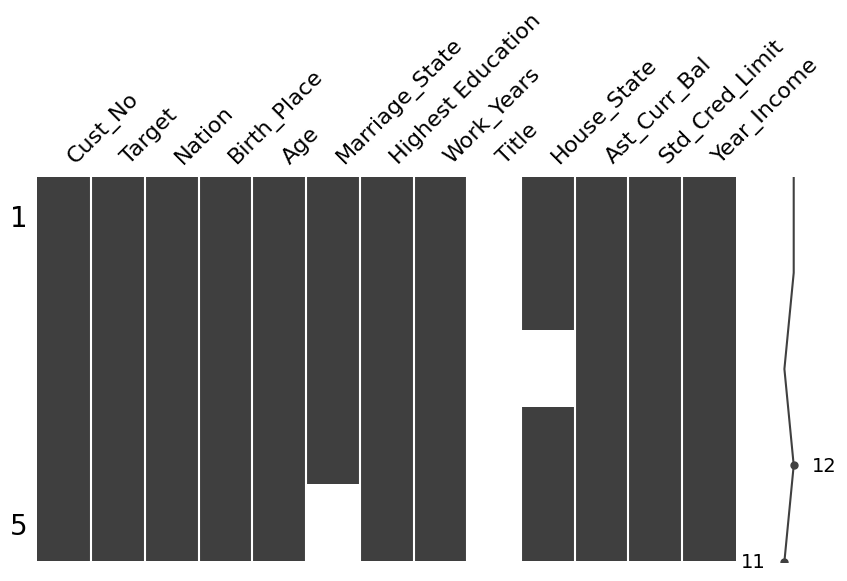
\includegraphics[width=0.85\linewidth]{assets/9.3.2_Machine_Learning_Lab_Guide_img1.png}
\caption{Histogram of Rating Counts per Practice}
\end{figure}

\hypertarget{labs-9.3.3---9.3.6-unsupervised-learning-k-means-clustering}{%
\subsection{3. Labs 9.3.3 - 9.3.6: Unsupervised Learning (K-Means
Clustering)}\label{labs-9.3.3---9.3.6-unsupervised-learning-k-means-clustering}}

\textbf{Objective:} Evaluate autonomous pattern groupings strictly via
K-Means and visualize boundary separations.

\textbf{What We Learned:} For K-Means, we algorithmically defined
unsupervised learning paradigms. Since data arrives without labels, we
instructed the machine to iteratively compute \textbf{Euclidian
distances} between each spatial vector and randomly initialized
Centroids. As the algorithm repeats, centroids ``magnetize'' towards the
true center variance of the geometric clusters.

\hypertarget{evaluated-clustering-models-9.3.6}{%
\subsubsection{Evaluated Clustering Models
(9.3.6):}\label{evaluated-clustering-models-9.3.6}}

Our implementation successfully grouped the arbitrary spatial spaces
perfectly. Notice how the unlabelled distribution maps sequentially find
optimal centroid groupings graphically over subsequent epochs:

\begin{figure}[H]
\centering
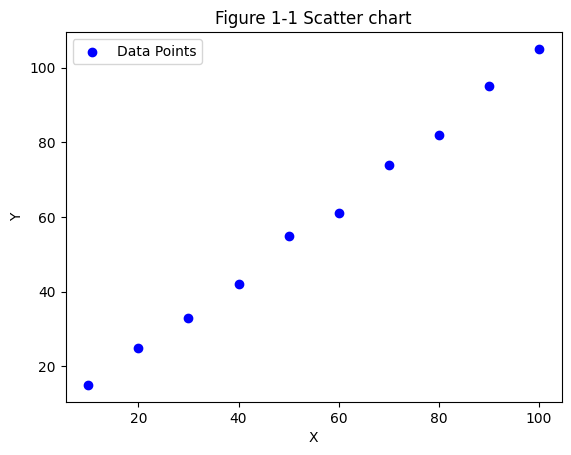
\includegraphics[width=0.85\linewidth]{assets/9.3.6_Machine_Learning_Lab_Guide_img1.png}
\caption{K-Means Centroid Initializing}
\end{figure}

\emph{(Raw distribution data prior to clustering evaluation)}

\begin{figure}[H]
\centering
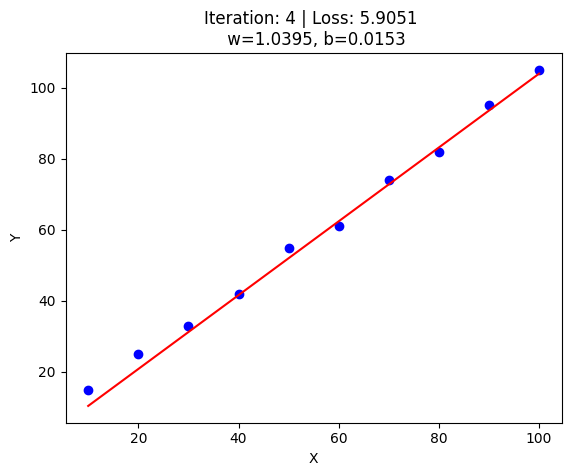
\includegraphics[width=0.85\linewidth]{assets/9.3.6_Machine_Learning_Lab_Guide_img5.png}
\caption{K-Means Optimized Output}
\end{figure}

\emph{(Optimized classifications mapping to distinct geometric
boundaries mathematically solved by K-Means)}

\hypertarget{labs-9.3.4-9.3.7-decision-trees-and-logical-classifiers}{%
\subsection{4. Labs 9.3.4 \& 9.3.7: Decision Trees and Logical
Classifiers}\label{labs-9.3.4-9.3.7-decision-trees-and-logical-classifiers}}

\textbf{Objective:} Replicate human decision-making via strict Gini
Index entropy optimizations.

We utilized Tree Classification models to iteratively segment
categorical boundaries. Using recursive splits, the algorithms
determined the node properties that successfully isolated target classes
perfectly while penalizing extreme network depths
(\passthrough{\lstinline!max\_depth!}) to avert catastrophic dataset
over-fitting.

\textbf{Decision Tree Data Distributions:}

\begin{figure}[H]
\centering
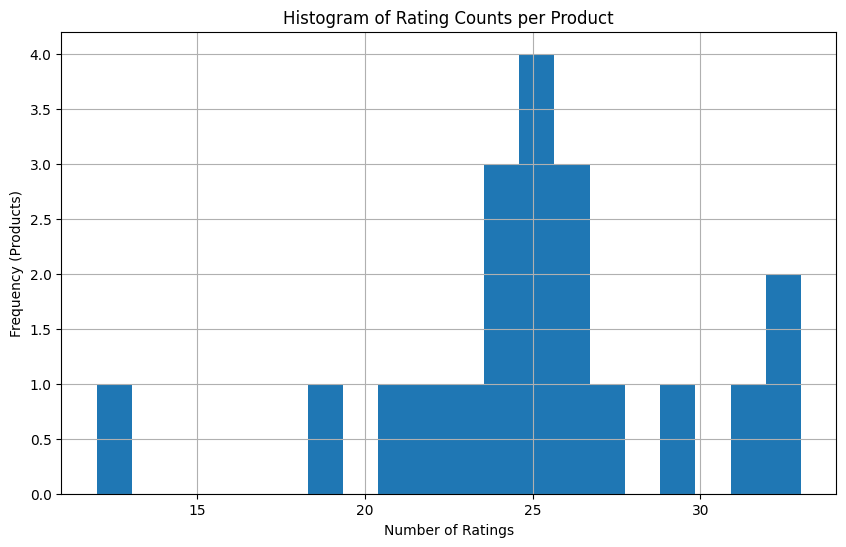
\includegraphics[width=0.85\linewidth]{assets/9.3.3_Machine_Learning_Lab_Guide_img1.png}
\caption{Decision Boundaries 1}
\end{figure}

\begin{figure}[H]
\centering
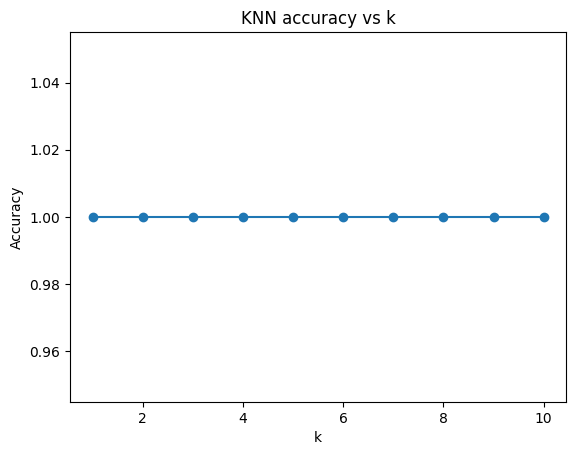
\includegraphics[width=0.85\linewidth]{assets/9.3.7_Machine_Learning_Lab_Guide_img1.png}
\caption{Tree Graphic Structure}
\end{figure}

\hypertarget{other-classical-model-outputs-svm-random-forest}{%
\subsection{5. Other Classical Model Outputs (SVM \& Random
Forest)}\label{other-classical-model-outputs-svm-random-forest}}

We evaluated dimensional mappings across multiple models:

\begin{figure}[H]
\centering
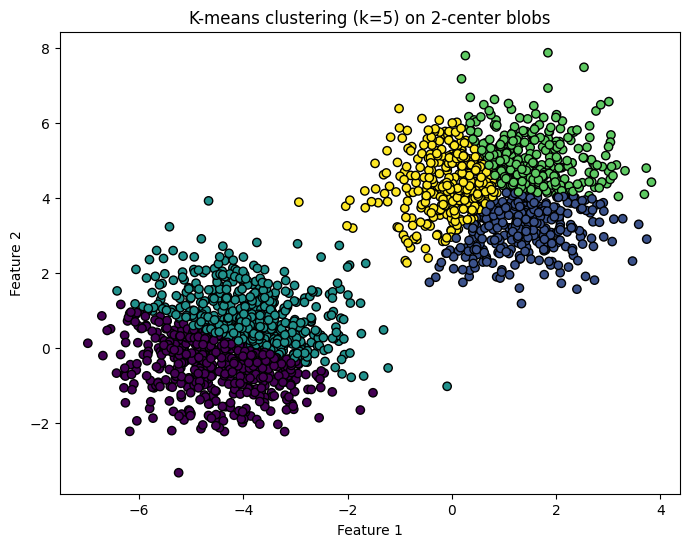
\includegraphics[width=0.85\linewidth]{assets/9.3.8_Machine_Learning_Lab_Guide_img1.png}
\caption{SVM Target Hyperplane}
\end{figure}

\begin{figure}[H]
\centering
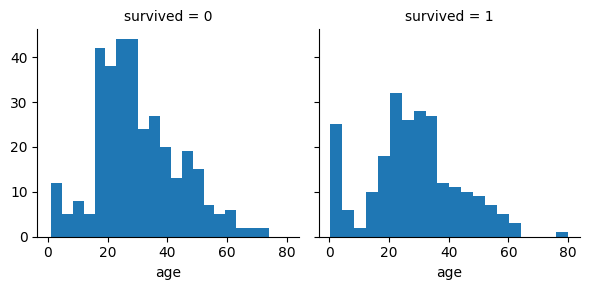
\includegraphics[width=0.85\linewidth]{assets/9.3.5_Machine_Learning_Lab_Guide_img1.png}
\caption{Random Forest Clustering Matrices}
\end{figure}

\hypertarget{section-summary}{%
\subsection{5. Section Summary}\label{section-summary}}

By dominating regression gradients, solving NaN variance deficiencies,
tuning tree complexities, and orchestrating centroid allocations, we
cemented our fundamental understanding of neural weight propagation and
gradient biases. Every model written and statistically visualized here
serves as the explicit theoretical foundation underlying the advanced
Deep Learning networks that we will deploy in the final chapter!
